\chapter{Zeitreisen\label{chapter:thema}}
\lhead{Zeitreisen}
\begin{refsection}
\chapterauthor{Sascha Jecklin und Jonas Gründler}
\section{Einleitung}

	Das Thema Zeitreisen fasziniert den Menschen, seit er sich der Zeit bewusst ist. Früh entstanden Träume, den Verlauf der Zeit manipulieren zu können. Erste schriftliche und bildliche Belege dafür gab es bereits in der hinduistischen Mythologie und in der buddhistischen Religion. Auch in der modernen Literatur und in der Filmindustrie sind Zeitreisen ein beliebtes Thema. Einige Beispiele daf\"ur sind: 
\begin{itemize}
    \item Time Machine, H.G.Wells, 1895 
    \item Das Ende der Ewigkeit, Isaac Asimov, 1955
    \item Back to the Future, 1985-1990
    \item Star Trek
    \item Doctor Who
    \item Interstellar
    \item \dots

\end{itemize}
In diesem Kapitel beschäftigen wir uns mit der mathematischen Beschreibung von Zeitreisen; wie man solche Effekte erreichen kann und ob sie mit heutigen Mitteln erreichbar sind. Zu beginn soll gezeigt werden, wie man eine Zeitreise mit Hilfe der Eigenzeit beschreibt.
Doch was ist genau die Eigenzeit? 
Die Eigenzeit ist die Geschwindigkeit mit der eine Uhr an Bord eines bewegten Objektes geht(Eigenzeit), im Vergleich zu einer relativ dazu unbewegten Uhr(Koordinatenzeit). 
Es zeigt sich das dies mit Gravitation und Geschwindigkeit möglich ist. Ein besonderes Augenmerk gilt dabei schwarzen Löchern. Nach dem wir die nötige Mathematik eingeführt haben, veranschaulichen wir das Ganze mit einer Simulation. Natürlich wollen wir uns auch Gedanken über die Realisierbarkeit machen. Wie sich zeigen wird, scheinen Zeitreisen keine reine Fiktion zu sein. Allerdings sind sie auch nicht in einem Ausmass möglich, wie man sich vielleicht erhofft.

\section{Was ist eine Zeitreise?}\label{}

Um diese Frage besser beantworten zu können, starten wir mit einem Gedankenexperiment. Wir stellen uns vor, zwei Autos fahren mit der gleichen Geschwindigkeit aneinander vorbei. Fahren die beiden Autos z.B. 100km/h schnell, ist die Relativgeschwindigkeit, mit der sie sich passieren gerade doppelt so hoch, also 200 km/h. In der klassischen Physik wäre das ein korrektes Ergebnis. In einem zweiten Anlauf sollen beide Fahrer Lichtgeschwindigkeit fahren. Spätestens jetzt macht sich ein Fehler bemerkbar. Denn die relative Geschwindigkeit, in der sich die beiden Fahrzeuge kreuzen ist nicht etwa doppelte Lichtgeschwindigkeit, sondern einfache Lichtgeschwindigkeit. Denn wir wissen das dies die grösste erreichbare Geschwindigkeit ist.
Beide Fahrer behaupten nun aber vehement, ihre eigene Geschwindigkeitsmessung sei korrekt gewesen. Folglich muss es Unterschiede in der Längen- und Zeitmessung geben.
Wie wir in Kapitel \ref{chap:lorentz} festgehalten haben, ist dies auch der Fall. Jeder Beobachter misst die gleiche Lichtgeschwindigkeit. Längen- und Zeitmessung muss in einem solchen System jedoch angepasst werden.

\subsection{Die Lorentz-Transformation}

Genau dies tun wir mit der Lorentz-Transformation aus Kapitel \ref{chap:lorentz}. Folglich gibt es nicht mehr "die Eine", allgemeine Zeitmessung" für alle Objekte. Jedes Objekt hat seine eigene Zeit, die sogenannte Eigenzeit.
Integrieren wir entlang einer Weltenlinie erhalten wir für die Eigenzeit:
\begin{equation}\label{Eigenzeit}
\tau
=
\int_{}^{}\frac{1}{\gamma}\,dt=\int_{}^{}\sqrt{1-\frac{v^2}{c^2}}\,dt
=
\frac{1}{c}\int_{}^{}\sqrt{g_{\mu\nu}\dot{x}^{\mu}(s)\dot{x}^{\nu}(s)}\,ds.
\end{equation}
Welche für jedes Objekt entsprechend ihrer Geschwindigkeit anders ist.
Da wir nun für jedes Objekt eine Eigenzeit festhalten, können wir auch Unterschiede dieser Zeiten angeben.
Eine Zeitreise beschreibt daher eine Bewegung durch die Zeit, abweichend von der eines Bezugssystems. 
Nicht nur hohe Geschwindigkeiten bringen Änderungen in der Zeitmessung. Wie wir sehen werden, verursachen auch andere Ursachen Dehnungen der Zeit. Der Effekte der verlangsamten Eigenzeit, heisst auch Zeitdilatation.
Streng genommen, bringt schon jede kleinste Geschwindigkeit eine Änderung der Eigenzeit. Da die praktische Anwendung in diesem Kapitel im Vordergrund steht, interessieren uns natürlich in erster Linie signifikante Unterschiede. Erst doppelt oder sogar zehnmal schneller vergehende Eigenzeiten w\"urden uns Effekte best\"atigen, welche man uns in Science Fiction Filmen und Romanen verspricht.

\subsection{Zukunft und Vergangenheit}

Es stellt sich noch die Frage, ob das nun Reisen in die Zukunft oder in die Vergangenheit sind. Beide unterscheiden sich Grundlegend voneinander.

\subsubsection{Vergangenheit}

Generell sind Reisen in die Vergangenheit sehr schwierig. Denn dort können Kausalitätsprobleme auftreten. Was z.B geschieht, wenn ein Zeitreisender seine Entstehung verhindern würde? Diese Frage lässt sich im Moment nicht beantworten, weil man schlicht und einfach nicht weiss, was passieren würde. Diese eher philosophischen Probleme, plus die Technische Umsetzbarkeit verhindern momentan eine Reise in die Vergangenheit.

\subsubsection{Zukunft}

%Vorschlag Jonas
Mit unterschiedlich schnell verlaufenden Eigenzeiten beschreibt man salopp ausgedrückt Reisen in die Zukunft oder "weniger schnelles altern". Ein Beobachter $A$ mit halb so schnell verlaufender Eigenzeit wie eine Referenz $B$ wäre quasi in die Zukunft gereist.
Ein Beobachter $A$ reist mit hoher Geschwindigkeit ein Jahr durch das Weltall. Für Beobachter $B$, welcher auf der Erde geblieben ist, vergehen in dieser Zeit zwei Jahre. Wenn $A$ also zurückkehrt ist er ein Jahr weniger alt als $B$ und somit in die Zukunft gereist. $A$ hat ein ganzes Jahr überbrückt. Aus der Sicht von $B$ ist $A$ also weniger schnell gealtert. Dazu kommt dass keiner in die Vergangenheit gereist ist, da beide trotz unterschiedlicher Eigenzeiten, älter geworden sind.

%original
%Mit unterschiedlich schnell verlaufenden Eigenzeiten beschreibt man salopp ausgedrückt Reisen in die Zukunft oder "weniger schnelles altern". Ein Beobachter A mit halb so grosser Eigenzeit wie eine Referenz B wäre quasi in die Zukunft gereist. Während für A ganz normal ein Jahr verstrich, wären für B zwei Jahre vergangen. Umgekehrt ist aus Sicht von B A weniger schnell gealtert. A ist damit aber nicht in die Vergangenheit gereist und kann trotz Zeit\"anderung immer nur älter sein als zu Beginn der Betrachtung.

\section{Einfluss von Geschwindigkeit und Gravitation}

Da wir nun Wissen, wie wir eine Zeitreise beschreiben können, müssen wir uns nun Gedanken machen, wie wir Zeitdilation erreichen können. Im wesentlichen gelingt dies durch Geschwindigkeit oder Gravitation. 
\subsection{Geschwindigkeit}
Hohe Geschwindigkeit ist eine Möglichkeit, Zeitdilatationen zu erreichen. Wenn sich eine Person relativ zu einem Bezugssystem schnell bewegt, vergeht f\"ur diese Person die Zeit im Vergleich zum Bezugssystem langsamer. Die Ver\"anderung wird durch den Lorentzfaktor beschrieben, welcher sich aus der Lorentztransformation herleiten l\"asst. Er beschreibt wie stark die Eigenzeit im Verhältnis zu einem Bezugssystem gedehnt wird. %corrected^^
\begin{equation} \label{lorentzfaktor}
    \gamma=\frac{1}{\sqrt{1-\displaystyle\frac{v^2}{c^2}}} 
\end{equation}
Dieses $\gamma$ kommt wie oben bei der Rechnung gezeigt und auch beschrieben, in der Berechnung der Eigenzeit vor. %angepasst
Die Formel \eqref{Eigenzeit} ist in dieser Form noch nicht sehr anschaulich. Sie zeigt jedoch, dass die jeweils gewählte Metrik mit den jeweiligen Basisvektoren "multipliziert" werden muss (Einsteinsche Summenkonvention). Je nach Metrik können andere Resultate entstehen.
Durch das Verwenden der Minkowski-Metrik, welche Raum und Zeit miteinander verbindet, und der Koordinaten $t, x, y, z$ l\"asst sich eine verst\"andliche Form herleiten. 
\begin{equation}
    g_{\mu\nu}=
    \begin{pmatrix}
        -1 & 0 & 0 & 0 \\
        0 & 1 & 0 & 0 \\
        0 & 0 & 1 & 0 \\
        0 & 0 & 0 & 1
    \end{pmatrix}
\end{equation}
Standard Vierervektor:
\begin{align*}
x^{0}=ct,\, x^{1}=x,\, x^{2}=y,\, x^{3}=z 
\end{align*}
Aus diesen Koordinaten kann man nun mittels Ableiten die Geschwindigkeiten bilden und in $v$ einsetzen.
Daraus Bildet sich eine Eigenzeitformel auf Basis der Minkowski-Metrik.
%corrected
\begin{align*}
    \tau
    =
    \frac{1}{c}\int_{}^{}\sqrt{-(-c^2\dot{t}(s)^{2}+\dot{x}(s)^{2}+\dot{y}(s)^{2}+\dot{z}(s)^{2})}\,ds
\end{align*}
Andere Metriken beschreiben andere Verläufe der Eigenzeit, da je nach Metrik unterschiedliche Räume und Faktoren in die Berechnung mit einbezogen werden. 
Je nachdem wie die Bewegung gew\"ahlt wird, können Koordinaten $x, y, z$ wegfallen.
Hier ein Beispiel bei welchem nur eine Geschwindigkeit in x-Richtung vorhanden ist ($c =$ Lichtgeschwindigkeit, $u$ beschreibt den Bruchteil von $c$)
\begin{align*}
     t(s)= s,\,
 	 x(s)=u\cdot c \cdot s,\,
     y(s)=0,\,
     z(s)=0 
\end{align*}
\begin{align*}
     \dot{t}(s)=1,\,
     \dot{x}(s)=u\cdot c,\,
     \dot{y}(s)=0,\,
     \dot{z}(s)=0
\end{align*}
Diese Koordinaten in das Integral eingesetzt ergeben folgende Form,
\begin{align*}
\tau
&=
\frac{1}{c}\int_{}^{}\sqrt{-(-c^2\dot{t}(s)^2+\dot{x}(s)^2)}\,ds 
=
\frac{1}{c}\int_{}^{}\sqrt{-(-c^2 +(u\cdot c)^{2}}\,ds\\
&=
\frac{s\sqrt{c^2+(u\cdot c)^{2}}}{c} 
=
s\sqrt{1-\frac{u^2\cdot c^2}{c^2}}
\end{align*}
welche eine einfache Form einer Zeitdilatation darstellt. Durch die Vereinfachung und das einsetzen der Werte entsteht also eine Form, welche dem Lorentzfaktor \eqref{lorentzfaktor} oben entspricht.
$u$ ist lediglich ein Parameter der zeigt mit welchem Bruchteil der Lichtgeschwindigkeit sich das Objekt bewegt.

\subsubsection{Beispiel}

Hier ein Zahlenbeispiel mit 20\% Lichtgeschwindigkeit:
$s=5000, u=0.2$ 
\begin{align*}
    t(s)=s,\,
    x(s)=0.2c \cdot s,\,
    y(s)=0,\,
    z(s)=0 
    \\
    \dot{t}(s)=1,\,
    \dot{x}(s)=0.2c,\,
    \dot{y}(s)=0,\,
    \dot{z}(s)=0
\end{align*}
Diese Werte in die Gleichung eingesetzt ergeben
\begin{align*}
 \tau
&=
\frac{1}{c}\int_{0}^{5000}\sqrt{-(-c^2\dot{t}(s)^2+\dot{x}(s)^2)}\,ds
=
\frac{1}{c}\int_{0}^{5000}\sqrt{-(-c^2+((0.2c)^2))}\,ds\\
&=
5000\sqrt{1-\frac{(0.2)^2 c^2}{c^2}} 
=
5000\sqrt{1-(0.2)^2}
=
4898.98
\end{align*}

\subsubsection{Der Lorentzfaktor in Abhängigkeit von $v$}

In Abbildung \ref{skript:zeitreisen:fig:lorentz} sieht man den Zusammenhang zwischen Geschwindigkeit und Lorentzfaktor als Graph. Obiges Beispiel und die Abbildung zeigen, dass eine relevante Zeitdilatation erst bei sehr hohen Geschwindigkeiten erreicht wird. Um wirklich grosse Zeitdilatationen zu erreichen, braucht man annähernd Lichtgeschwindigkeit. Wie bald ersichtlich wird, stellt dies ein gravierendes Problem bei der Realisierung dar.
\begin{figure}[H]
    \centering
    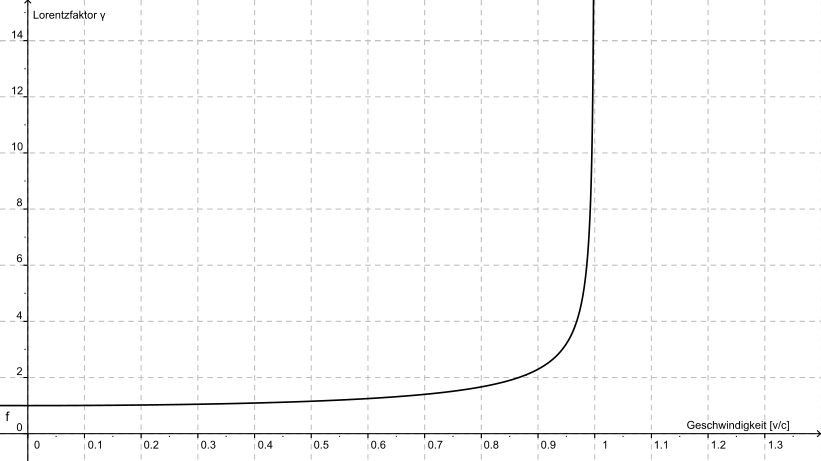
\includegraphics[width=\hsize]{zeitreisen/Lorentzfaktor.jpg}
    \caption{Änderung des Lorentzfaktors in Abh\"angigkeit der Geschwindigkeit}
        \label{skript:zeitreisen:fig:lorentz} 
\end{figure}
\subsection{Gravitation} \label{Gravitation}

	In diesem Kapitel beschäftigen wir uns mit dem Einfluss der Gravitation auf die Zeit. Einstein hat erkannt, dass die Gravitation durch eine Krümmung des Raumes beschrieben werden muss. Erkennen lässt sich die Gravitation z.B. an der Erdbeschleunigung. Alles wird mit $g=9.81\frac{m}{s^2}$ in Richtung Erdmittelpunkt beschleunigt. $F=\frac{KMm}{r^2}$. F lässt sich jedoch nach dem zweiten Newtonschen Gesetz auch als $F=m\cdot a$ schreiben. Eingesetzt und gekürzt zeigt sich, dass die Beschleunigung nicht von der Masse des betrachteten Objektes abhängt.
	\begin{align*}
		m\cdot a = \frac{KMm}{r^2} \Leftrightarrow a=\frac{KM}{r^2} 
	\end{align*}
	Dieser Effekt lässt sich auch im Alltag betrachten. Grosse fallende Objekte werden gleich stark richtung Erdmittelpunkt beschleunigt wie kleine.
	
	\subsubsection{Koordinatentransformationen}
	
	Die folgenden Gleichungen sind zwar eine Koordinatentransformation, doch sie sind keine Lorentztransformation und enthalten somit die Minkowski-Metrik nicht. Mit ihr lässt sich der Einfluss der Gravitation auf die Zeit nicht berechnen. 
	
	\begin{equation}
	\left.
	\begin{aligned}
	t'&=t\\
	x'&=x+\frac12gt^2
	\end{aligned}
	\right\}
	\qquad
	\Leftrightarrow
	\qquad
	\left\{
	\begin{aligned}
	t&=t'\\
	x&=x'-\frac12gt'^2
	\end{aligned}
	\right.
	%\eqref{skript:gravitation:beschleunigt}
	\end{equation}
	Das $t'$ entspricht immer noch $t$ obwohl eine Transformation durchgeführt wurde. 
	Der Ansatz $ -c^2dt^2 + dx^2 + dy^2 + dz^2$ genügt also nicht mehr. Wir müssen also Metriken und Transformationen zulassen, welche von der Minkowski-Metrik und der Standarttransformation abweichen.
	
	\subsubsection{Metriken}
	
	Doch welche Metrik beinhaltet den Einfluss der Gravitation auf die Zeit? 
	Da der Raum durch die Gravitation gekrümmt wird, benötigen wir ein Metrik und auch eine Längenmessung, welche gravitative Effekte miteinbezieht.
	Zum Glück kennen wir bereits eine solche Metrik. Die Schwarzschild-Metrik eignet bestens dazu, denn sie beschreibt die Raumkrümmung um massereiche Objekte. Wir werden sie später auf ein schwarzes Loch anwenden. Allerdings nehmen wir an, dass diese nicht rotieren und auch keine Ladung besitzen. Dadurch nehmen wir zwar Fehler in Kauf, dafür hält sich der rechnerische Aufwand in Grenzen. Um diese weiteren Effekte miteinzubeziehen wird die Kerr- oder die Kerr-Newman Metrik benötigt. Doch das Rechnen mit diesen Metriken ist um ein vielfaches komplizierter und ausserhalb unserer Möglichkeiten. Deshalb beschränken wir uns auf die Schwarzschild-Metrik.

	\section{Realisierbarkeit}
    
    Theoretisch sind Zeitreisen also umsetzbar. Nun gilt es zu prüfen, inwiefern so etwas in der Praxis möglich ist. Es gibt jedoch mehrere Probleme, die eine Zeitreise verhindern können.
    Betrachten wir zuerst grosse Geschwindigkeiten. Wie wir in Abbildung \ref{skript:zeitreisen:fig:lorentz} bereits gesehen haben, treten die gewünschten Effekte erst bei vergleichbar grossen Geschwindigkeiten auf. Ab $0.99c$ beginnt der Faktor $\gamma$ stark zu wachsen und die Zeitdilatation würde für uns akzeptable Werte erreichen.
    Doch wie lässt sich diese Geschwinigkeit überhaupt erreichen?
    
    \subsubsection{Energie}\label{skript:chapters:zrirtreisen:energie}
    
    Doch wie aus der Physik bekannt ist, berechnet sich die kinetische Energie eines Objekts aus $E_{\text{kin}}=\frac{1}{2}mv^2$. Doch der Faktor $c^2$ lässt die kinetische Energie auch für verschwindend kleine Massen ins unerreichbare schnellen.
    In aktuellen wissenschaftlichen Experimenten, plant man, kleine Segel mittels Laserstrahlen auf 20\% Lichtgeschwindigkeit zu beschleunigen. Bis der Mensch und seine Fortbewegungsmittel also solche Geschwindigkeiten erreichen und die dafür benötigte Energie zur Verfügung stellen können, wird noch einige Zeit vergehen.
    Das bedeutet also, dass mittels Geschwindigkeit in naher Zukunft keine signifikanten Zeitdilatationen erreicht werden können. Auch wenn der Effekt in gewissen Präzisionsanwendungen berücksichtigt werden muss, ist er für uns anders als eigentlich Erwartet relevant. Bleibt zu hoffen, dass die Gravitation bessere Resultate bringt. 
    
    \subsubsection{Massereiche Objekte}
    
    Um also eine Zeitdilatation zu erreichen, müssen wir auf Die Gravitation ausweichen. Betrachten wir als nächstes die Erde. Die Gravitation der Erde beeinflusst die Zeit in GPS-Satelliten bereits derart, dass die resultierenden Fehler mathematisch herausgerechnet werden müssen. Nachzulesen in Kapitel \ref{chap:gps} %Wie got das genau?. Das machi no wenns online isch.
    Da der Effekt jedoch zu klein ist für eine wirkliche Zeitreise, lässt sich die gleiche Rechnung mit der Sonne machen. Schnell wird klar, dass selbst die grössten Sterne zu wenig Masse haben, um eine nennenswerte Zeitdilatation zu verursachen. Unsere Simulationen Zeigen, dass selbst riesige Sonnen einen zu kleinen Effekt auf die Zeit haben
    %simulation rg_erde = 8.8mm Geostationärer orbit 35800km -> effekt = 0...
    Benötigt werden also schwere Objekte an die man, im besten Fall, auch nahe heran fliegen kann. Das Ergebnis aus diesem Ausschlussverfahren sind deshalb, als letzte Option, schwarze Löcher. Von unserer Position aus gesehen ist das nächste schwarze Loch Sagittarrius A*, welches sich im Zentrum unserer Galaxis befindet. Dieses supermassive schwarze Loch sollte den Anforderungen genügen. Unsere späteren Simulationen werden auch zeigen, dass sich mittels Sagittarrius A* tatsächlich eine signifikante Zeitdilatation erreichen lässt.
    
    \subsection{Reise}
    
    Doch hier beginnen auch neue Probleme. Sagittarrius A* ist 26000 Lichtjahre von uns entfernt. Das bedeutet, auch mit Lichtgeschwindigkeit benötigen wir 26000 Jahre um dort anzukommen. Die grosse Hoffnung ist, dass wir durch eine hohe Fluggeschwindigkeit und die daraus resultierende Zeitdilatation die Eigenzeit, an Bord des Raumschiffes, verkürzen können. 
    Doch wie bereits oben erwähnt, lässt sich eine für unsere Zwecke ausreichende Zeitdilatation erst mit sehr hohen Geschwindigkeiten erreichen. Wie bereits oben beschrieben, sind solche hohen Geschwindigkeiten momentan nicht möglich.
    Hier eine Beispielrechnung, in welcher wir mit einer Geschwindigkeit von $0.5c$ fliegen.
	\begin{align*}
	\tau
	&= 
	\int_{}^{26000}\frac{1}{\gamma}dt=\int_{}^{26000}\sqrt{1-\frac{v^2}{c^2}}\,dt
	= 
	\frac{1}{c}\int_{0}^{26000}\sqrt{-(-c^2+(0.5c)^2)}\,ds\\
	&=
	\biggl[s\sqrt{1-\frac{(0.5c)^{2}}{c^2}}\biggr]_0^{26000}
	=
	22516.7
	\end{align*}
	Wir benötigen für die Strecke also ca. 22500 Jahre.
	Folgende Tabelle zeigt die Eigenzeit im reisenden Raumschiff abhängig von der Geschwindigkeit.
	
	\begin{center}
		\begin{tabular}{ | l | p{5cm} |}
			\hline
			Geschwindigkeit & Eigenzeit im Raumschiff \\ \hline
			$20\%c$ & 25474.5 Jahre \\ \hline
			$50\%c$ & 22516.7 Jahre \\ \hline
			$80\%c$ & 15600 Jahre \\ \hline
			$99\%c$ & 3667.75 Jahre \\ \hline
			$99.99\%c$ & 367.686 Jahre \\ \hline
			$99.9999\%c$ & 36.76 Jahre \\ \hline
			$99.999999\%c$ & 3.6 Jahre \\ \hline
		\end{tabular}
	\end{center}
	Wie die Tabelle zeigt, würde auch ein Flug mit $0.99c$ noch viel zu lange dauern. 
	Die Eigenzeit im Raumschiff beträgt zwar nur noch einen Bruchteil der von aussen gesehenen Reisezeit, jedoch ist es trotz dieser Zeiteinsparnis nicht möglich so das Ziel zu erreichen.
	Wir müssen mit unserem Projekt also warten, bis mit Raumschiffen annähernd Lichtgeschwindigkeit erreicht werden kann. Zusätzlich muss auch noch das oben genannte Energieproblem gelöst werden (Abschnitt \ref{skript:chapters:zrirtreisen:energie}). Es muss ein Treibstoff mit grosser Energiedichte gefunden werden, sodass nicht riesige Mengen an Treibstoff mit befördert werden müssen. Dies würde die Masse des Raumschiffes zusätzlich erhöhen und dadurch auch wieder die benötigte Energie vergrössern. Ein Teufelskreis.
	Wir verschieben unser Projekt also in hypothetische und stellen uns vor, wir wären bereits da.
	
	\subsection{Am Ziel\dots Was nun?}
	
	Wenn wir nun also diese Reise auf uns genommen haben, und Sagittarrius A* wirklich erreichen, eröffnen sich uns zwei Möglichkeiten:
	\begin{itemize}
		\item eine gesteuerte Bahn
		\item wir lassen uns "fallen"
	\end{itemize}
	In den folgenden Abschnitten werden die Vor- und Nachteile der jeweiligen Methoden beschrieben.
	
	\subsubsection{Eine Gesteuerte Bahn}
	Eine gesteuerte Kreisbahn um das schwarze Loch bringt die besten Resultate, da wir eine Kreisbahn sehr nahe am Ereignishorizont wählen können. Denn je näher wir uns am Ereignishorizont befinden, desto stärker sind die Auswirkungen auf die Zeit. 
	Um jedoch einen konstanten und nahen Orbit am schwarzen Loch zu fliegen , muss das Raumschiff in der Lage sein, der Gravitation zu widerstehen. Das liesse sich auf zwei Arten erreichen. Entweder mittels einer Hohen Geschwindigkeit, bei welcher die Fliehkraft des Raumschiffs der Gravitation entgegenwirkt. Oder mit langsamerer Geschwindigkeit, bei welcher der Gravitationskraft mittels Steuerdüsen entgegengewirkt wird. 
	Beide Methoden benötigen sehr viel Energie, und sind deshalb keine Option. Der grösste Teil des Treibstoffes wurde bereits während der Reise  verbraucht.
	%Rückreise?
	\subsubsection{Wir lassen uns "fallen"}
	
	Die zweite Möglichkeit wäre, dass wir uns, wenn wir angekommen sind "fallenlassen" und sehen was passiert. So können je nach Anfangsgeschwindigkeit, Abstand und Position verschiedene Bahnen erreicht werden. Die Geschwindigkeit, Richtung und Abstand vom schwarzen Loch stellen Bei der Ankunft also gerade die Anfangsbedingungen dar. Vom Absturz in den Ereignishorizont, bis zu einer Bahn auf der wir dem Gravitationstrichter des schwarzen Lochs entkommen und uns in die weiten des Weltalls verabschieden ist alles möglich. Beides sind jedoch eher unangenehme Szenarien. 
	Wie findet man also eine Bahn möglichst nahe am schwarzen Loch, ohne dass eines dieser zwei Ereignisse eintritt und ohne weitere Steuerenergie zu verwenden?
	Lösung unseres Problem sind die Geodätengleichungen, welche uns aufgrund der Anfangsbedingungen eine Bahn berechnen lassen. Aus der Lösung dieser Gleichungen lässt sich dann auch die Eigenzeit und somit die Effizienz unserer Zeitreise berechnen. Dies werden wir am Schluss der Arbeit mittels einer Simulation durchführen, und so sehen, wie viel Zeit wir tatsächlich einsparen können.
	
	\section{Umsetzung mittels Geodätenbahnen}
	
	Mit den Geodäten lassen sich nun physikalisch korrekte Bahnen um ein schwarzes Loch herleiten. Dafür benötigen wir die in Kapitel \ref{chap:geodaeten}
	%funktioniert nöd
	vorgestellte Geodätengleichung:	
	\begin{equation}
	\ddot{x}^{\alpha} + \Gamma^{\alpha}_{\mu\nu}\dot{x}^{\mu}\dot{x}^{\nu} = 0
	\end{equation}
	Nun können in der nähe des schwarzen Lochs alle Antriebe ausgeschaltet werden. Die aktuelle Geschwindigkeit, Position, Richtung und Abstand stellen nun die Anfangsbedingungen dar. Daran dass die Gleichung $=0$ ist, können wir erkennen, dass kein weiterer Energieinput benötigt wird. Die Gleichungen berücksichtigen auch die Energieerhaltung und somit, wie sich das Raumschiff in Zukunft mit abgeschalteten Antrieben bewegen wird. Mit einer numerischen Lösung dieses Differentialgleichungssystems lassen sich nun Schritt für Schritt die neuen Faktoren ausrechnen. Wir werden im nächsten Kapitel sehen, dass dann die Zeit in der Simulation langsamer vergeht und wir so daraus die Zeitdilatation extrahieren können.
	Wir k\"onnen nun die Gleichung wie folgt umstellen:	
	\begin{equation}
	\ddot{x}^{\alpha} = -\Gamma^{\alpha}_{\mu\nu}\dot{x}^{\mu}\dot{x}^{\nu}
	\end{equation}
	Daraus lässt sich interpretieren, dass die Beschleunigungen, welche für die nächste Position wichtig sind, ein Produkt aus den Christoffelsymbole 2. Art und den zugehörigen Ableitungen sind. Die Christoffelsymbole sind die $\Gamma^{\alpha}_{\mu\nu}$. Sie beschreiben, wie sich die im Raumschiff enthaltene Energie transformiert, und sich so die Beschleunigungen in die jeweiligen Richtungen, die Geschwindigkeiten und die Position verändern. Zusätzlich beschreiben sie auch den Einfluss das Gravitationsfeldes auf unser Raumschiff.
	Doch woher kommen diese Symbole, und wie lassen sie sich berechnen?
	Sie errechnen sich aus der jeweilig gewählten Metrik. Wie bereits im Abschnitt \ref{Gravitation} über Gravitation angedeutet, benötigen Wir für unsere Zwecke die Schwarzschild-Metrik, da sie den Einfluss der Gravitation auf unser Raumschiff berücksichtigt. Die genaue Erklärung der Christoffelsymbole \ref{christoffel} und der Schwarzschildmetrik \ref{Schwarzschild-Metrik} folgen in den nächsten zwei Unterkapiteln.
	Nun lässt sich die Gleichung von oben in vier Komponenten aufspalten.
	Entsprechend dem gewählten Koordinatensystem teilt sie sich in vier Gleichungen auf.
	\begin{align*}
	\ddot{t}(s) = -\Gamma^{1}_{\mu\nu}\dot{x}^{\mu}\dot{x}^{\nu}
	\ddot{r}(s) = -\Gamma^{2}_{\mu\nu}\dot{x}^{\mu}\dot{x}^{\nu}\\
	\ddot{\vartheta}(s) = -\Gamma^{3}_{\mu\nu}\dot{x}^{\mu}\dot{x}^{\nu}\\
	\ddot{\varphi}(s) = -\Gamma^{4}_{\mu\nu}\dot{x}^{\mu}\dot{x}^{\nu}		
	\end{align*}
	Die Ähnlichkeiten zum Kugelkoordinatensystem sind ersichtlich und werden in Kapitel \ref{Schwarzschild-Metrik} genauer erklärt.
	Da wir uns in einer Ebene bewegen ist der Winkel$\vartheta = const$ und somit sind seine Ableitungen $=0$. Die dritte Gleichung reduziert sich also auf $\ddot{\vartheta}(s)=0$ und fällt somit weg. Das Problem reduziert sich also auf 3 Dimensionen.
	\begin{align*}
	\ddot{t}(s) = -\Gamma^{1}_{\mu\nu}\dot{x}^{\mu}\dot{x}^{\nu}\\
	\ddot{r}(s) = -\Gamma^{2}_{\mu\nu}\dot{x}^{\mu}\dot{x}^{\nu}\\
	\ddot{\varphi}(s) = -\Gamma^{4}_{\mu\nu}\dot{x}^{\mu}\dot{x}^{\nu}		
	\end{align*}
	Da nun alle Elemente bekannt sind, lässt sich folgendes Differentialgleichungssystem aufstellen:
	\begin{equation}
	\begin{aligned}
	\ddot t(s)
	&=
	-\frac{1}{1-\displaystyle\frac{r_g}{r}}\frac{r_g}{r}\frac{1}{r}\dot t(s)\,\dot r(s)
	\\
	\ddot r(s)
	&=
	-\biggl(1-\frac{r_g}{r}\biggr)\frac{r_g}{r}\frac1{2r}\dot t(s)^2
	+\frac{1}{1-\displaystyle\frac{r_g}{r}} \frac{r_g}{r}\frac1{2r}\dot r(s)^2
	- (r_g-r) \dot\varphi(s)^2
	\\
	\ddot \varphi(s)
	&=
	-\frac2r \dot r(s)\,\dot\varphi(s)
	\end{aligned}
	\end{equation}\label{finaleq}
	Dieses nichttriviale System lässt sich nur numerisch lösen. Im nächsten Kapitel werden die Gleichungen mittels einem Matlab-Simulationprogramm gelöst. Dann finden wir auch heraus, wie effizient Zeitreisen mittels schwarzer Löcher wirklich sind.
	
	\subsection{Schwarzschild-Metrik}\label{Schwarzschild-Metrik}
	
	Die Metrik welche von Karl Schwarzschild gefunden wurde, ist ein Lösung der Einsteinschen Feldgleichungen und wurde nur wenige Monate nach deren Vorstellung gefunden.
	Die Schwarzschildmetrik in Vektordarstellung:
	\begin{equation}
	g_{\mu\nu}=
	\begin{pmatrix}
	-\biggl(-1-\frac{r_{g}}{r}\biggr) & 0 & 0 & 0 \\
	0 & \frac{1}{\displaystyle1-\frac{r_{g}}{r}} & 0 & 0 \\
	0 & 0 & r^{2} & 0 \\
	0 & 0 & 0 & r^{2}\sin^{2}(\vartheta)
	\end{pmatrix}
	\end{equation}
	Dazu gehört folgender Vierervektor, welcher ein um die Zeit erweitertes Kugelkoordinatensystem beschreibt.
	\begin{align*}
	x^{0}=ct,
	x^{1}=r,
	x^{2}=\vartheta,
	x^{3}=\varphi
	\end{align*}
	Die Metrik lässt sich nun auch in Zeilenform darstellen. So geschrieben, stellt sie auch gleich die Längenmessung im betrachteten Raum dar.
	\begin{equation}
	ds^2
	=
	-\biggl(1-\frac{r_g}r\biggr)c^2\,dt^2
	+
	\frac{1}{\displaystyle 1-\frac{r_g}r}\,dr^2 
	+
	r^2d\vartheta^2 
	+ 
	r^2\sin^2(\vartheta)d\varphi
	\end{equation}
	$r_g$ beschreibt den Gravitationsradius(Ereignishorizont) des betrachteten Körpers.
	Sie berücksichtigt auch die Krümmung des Raumes, also die Gravitation, und ist so für unsere Zwecke bestens geeignet. Die Metrik beschreibt den Gravitationstrichter um ein ungeladenes, nicht rotierendes schwarzes Lochs, und ist somit die einfachste Lösung. Es gibt noch weiter Metriken, welche diese Faktoren ebenfalls berücksichtigen (Kapitel \ref{Gravitation}), doch diese werden nicht weiter betrachtet.
	Die Herleitung der Metrik sparen wir uns hier, der Prozess wird bereits in Kapitel \ref{skript:chapter:schwarzschild} beschrieben.
	\subsubsection{Bedeutung von $R_{g}$ und der Ereignishorizont}
	Der Ereignishorizont stellt in der allgemeinen Relativitätstheorie eine Grenzfläche dar. Er beschreibt die Entfernung ab welcher das Licht nicht mehr aus dem Gravitationstrichter entkommen kann. Teilchen, welche den Ereignishorizont passiert haben, können diesen nicht mehr verlassen. Alle Teilchen oder Objekte die den Ereignishorizont passieren werden unweigerlich ins Zentrum stürzen. Alles ausserhalb dieses Radius hätte die Möglichkeit zu entkommen, die Frage ist nur, wie viel Energie benötigt wird. Da sogar das Licht nicht mehr entkommt, nennt man diese Objekte auch schwarze Löcher oder Singularitäten.
	Der Gravitationsradius lässt sich wie folgt berechnen.
	\begin{equation} \label{Gravitationsradius}
	r_{g}= \frac{2MG}{c^2}
	\end{equation}
	Der Gravitationsradius der Erde beträgt etwa 8.8mm. Wenn wir die Erde also unter diese 8.8mm komprimieren, wäre sie kleiner als der Gravitationsradius und wäre so nicht mehr sichtbar.
	\subsection{Christoffelsymbole}\label{christoffel}
	Die Berechnung der Christoffelsymbole aus der Schwarzschild-Metrik ist kompliziert und sehr Rechenaufwändig. Wir beschränken uns hier auf die Berechnung, die Herleitung wird in Kapitel \ref{skript:chapters:geodaeten} ausführlich beschrieben. Es gibt Christoffelsymbole erster und zweiter Art, die Christoffelsymbole 2. Art lassen sich aus denen 1. Art berechnen.
	$g_{\mu\nu}$ ist hier die Schwarzschild-Metrik in Vektorform \ref{Schwarzschild-Metrik}.
	Die Christoffelsymbole 1. Art berechnen sich aus:
	\begin{equation}
	%\begin{align*}
		\Gamma_{\alpha,\mu\nu} 
		= 
		\frac{1}{2}\biggl(\frac{\partial g_{\nu\alpha}}{\partial x^{\mu}} 
		+
		\frac{\partial g_{\alpha\mu}}{\partial x^{\nu}}
		+
		\frac{\partial g_{\mu\nu}}{\partial x^{\alpha}}
		 \biggr)
	%\end{align*}
	\end{equation}
	Die Christoffelsymbole 2. Art:
	\begin{equation}
	%\begin{align*}
	\Gamma^{\sigma}_{\mu\nu} 
	= 
	g^{\sigma\alpha}\Gamma_{\alpha,\mu\nu} 
	=
	\frac{1}{2}g^{\sigma\alpha}\biggl(\frac{\partial g_{\nu\alpha}}{\partial x^{\mu}} 
	+
	\frac{\partial g_{\alpha\mu}}{\partial x^{\nu}}
	+
	\frac{\partial g_{\mu\nu}}{\partial x^{\alpha}}
	\biggr)
	%\end{align*}
	\end{equation}
	Sie werden Auch Zusammenhangskoeffizienten genannt.
	Folgende Christoffelsymbole entstehen nach einer Berechnung mit MAXIMA.
	%\begin{equation}
	\begin{align*}
	\Gamma^0_{01}
	&=
	\frac{1}{1-\displaystyle\frac{r_g}{r}}
	\frac{r_g}{r}
	\frac{1}{2r}
	\\
	\Gamma^1_{00}
	&=
	\biggl(1-\displaystyle\frac{r_g}{r}\biggr)
	\frac{r_g}{r}
	\frac{1}{2r}
	&
	\Gamma^1_{11}
	&=
	-\frac1{1-\displaystyle\frac{r_g}{r}}
	\frac{r_g}{r}
	\frac{1}{2r}
	&
	\Gamma^1_{22}
	&=
	r_g-r
	&
	\Gamma^1_{33}
	&=
	r_g-r
	\\
	\Gamma^2_{12}
	&=
	\frac1r
	\\
	\Gamma^3_{13}
	&=
	\frac1r
	\end{align*}
	%\end{equation}
	Theoretisch würden für ein vierdimensionales Koordinatensystem $4^{3}$ Christoffelsymbole entstehen. Die Berechnung hat jedoch gezeigt, dass der grösste Teil der Symbole zu $0$ wird und so aus der Gleichung \ref{finaleq} herausfallen. Was die Berechnung und Simulation um ein vielfaches erleichtert.
		
	\section{Simulation}
	
	%Erklärung sourcecode
	
	\section{Fazit}
	
	Welche Erkenntnisse ziehen wir also aus unserem Projekt?
	Wir haben herausgefunden, dass sich mittels der Gravitation eine Zeitreise erreichen lässt. Jedoch zeigen unsere Simulationen, dass es schwierig ist mehr als 20\% Zeitverlangsamung zu erreichen. Dass grösste Problem ist jedoch, überhaupt ein schwarzes Loch zu erreichen. Momentan scheitert das "Projekt Zeitreise" hauptsächlich daran. Auch mit 99\% Lichtgeschwindigkeit dauert es noch hunderte von Jahren, bis wir das Ziel, trotz Zeitdilatation, erreichen. Wir werden also warten müssen, bis die Wissenschaft einen Weg gefunden hat, diese Strecke in brauchbarer Zeit zu reisen, oder zu überbrücken. %Science-fiction lässt grüssen;)
	


	\printbibliography[heading=subbibliography]
	\end{refsection}

